\section{Performance \& GPU Optimization}

\begin{frame}
\frametitle{GPU Occupancy}

\begin{conceptbox}{GPU Execution Model}
\begin{itemize}
    \item \textbf{SIMD/SIMT}: Single Instruction, Multiple Threads
    \item \textbf{Warps/Wavefronts}: Groups of 32/64 threads execute together
    \item \textbf{Occupancy}: Ratio of active warps to maximum possible warps
\end{itemize}
\end{conceptbox}

\begin{center}
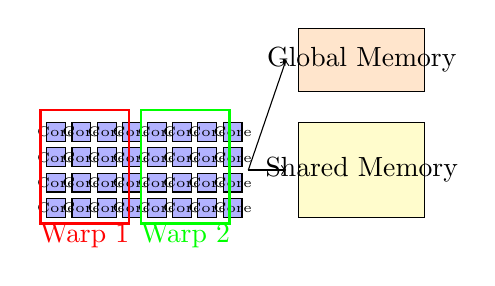
\begin{tikzpicture}[scale=0.8]
    % GPU cores representation
    \foreach \x in {0,...,7} {
        \foreach \y in {0,...,3} {
            \draw[fill=blue!30] (\x*0.4, \y*0.4) rectangle ++(0.3, 0.3);
            \node at (\x*0.4+0.15, \y*0.4+0.15) {\tiny Core};
        }
    }
    
    % Warp grouping
    \draw[red, thick] (-0.1, -0.1) rectangle (1.3, 1.7);
    \node[red] at (0.6, -0.3) {Warp 1};
    
    \draw[green, thick] (1.5, -0.1) rectangle (2.9, 1.7);
    \node[green] at (2.2, -0.3) {Warp 2};
    
    % Memory hierarchy
    \draw[fill=yellow!20] (4, 0) rectangle (6, 1.5);
    \node at (5, 0.75) {Shared Memory};
    
    \draw[fill=orange!20] (4, 2) rectangle (6, 3);
    \node at (5, 2.5) {Global Memory};
    
    \draw[->] (3.2, 0.75) -- (3.8, 0.75);
    \draw[->] (3.2, 0.75) -- (3.8, 2.5);
\end{tikzpicture}
\end{center}

\end{frame}

\begin{frame}
\frametitle{Memory Hierarchy \& Bandwidth}

\begin{center}
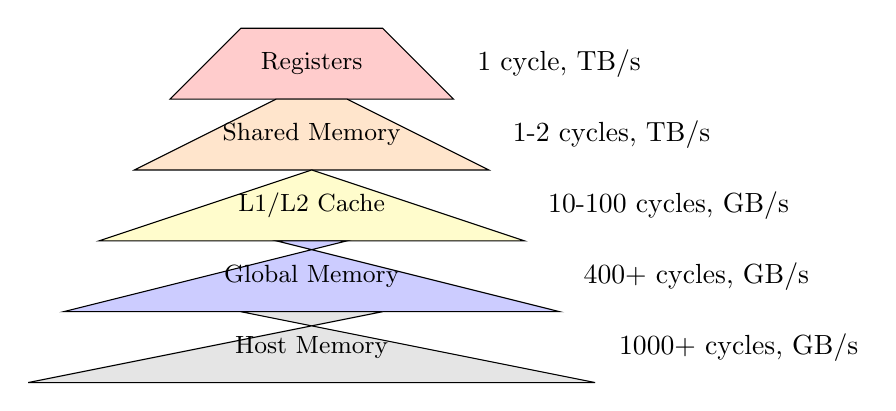
\begin{tikzpicture}[scale=0.9]
    % Memory pyramid
    \draw[fill=red!20] (0,4) -- (1,5) -- (3,5) -- (4,4) -- cycle;
    \node at (2,4.5) {\small Registers};
    \node[right] at (4.2,4.5) {1 cycle, TB/s};
    
    \draw[fill=orange!20] (-0.5,3) -- (1.5,4) -- (2.5,4) -- (4.5,3) -- cycle;
    \node at (2,3.5) {\small Shared Memory};
    \node[right] at (4.7,3.5) {1-2 cycles, TB/s};
    
    \draw[fill=yellow!20] (-1,2) -- (2,3) -- (2,3) -- (5,2) -- cycle;
    \node at (2,2.5) {\small L1/L2 Cache};
    \node[right] at (5.2,2.5) {10-100 cycles, GB/s};
    
    \draw[fill=blue!20] (-1.5,1) -- (2.5,2) -- (1.5,2) -- (5.5,1) -- cycle;
    \node at (2,1.5) {\small Global Memory};
    \node[right] at (5.7,1.5) {400+ cycles, GB/s};
    
    \draw[fill=gray!20] (-2,0) -- (3,1) -- (1,1) -- (6,0) -- cycle;
    \node at (2,0.5) {\small Host Memory};
    \node[right] at (6.2,0.5) {1000+ cycles, GB/s};
\end{tikzpicture}
\end{center}

\begin{mathbox}{Memory Optimization Strategies}
\begin{itemize}
    \item \textbf{Coalescing}: Align memory accesses to cache lines
    \item \textbf{Tiling}: Use shared memory for data reuse
    \item \textbf{Occupancy vs Resources}: Balance thread count with memory usage
\end{itemize}
\end{mathbox}

\end{frame}

\begin{frame}
\frametitle{Optimization Strategies}

\begin{columns}
\begin{column}{0.5\textwidth}
\begin{conceptbox}{Vertex Optimizations}
\begin{itemize}
    \item \textbf{Index buffers}: Reuse vertices
    \item \textbf{Vertex cache}: Post-transform vertex cache
    \item \textbf{Instancing}: Reduce draw calls
    \item \textbf{LOD}: Level of detail systems
\end{itemize}
\end{conceptbox}
\end{column}

\begin{column}{0.5\textwidth}
\begin{conceptbox}{Fragment Optimizations}
\begin{itemize}
    \item \textbf{Early-Z}: Reject occluded fragments
    \item \textbf{Z-prepass}: Render depth first
    \item \textbf{Culling}: Back-face, frustum, occlusion
    \item \textbf{Batching}: Minimize state changes
\end{itemize}
\end{conceptbox}
\end{column}
\end{columns}

\vspace{0.5cm}

\begin{center}
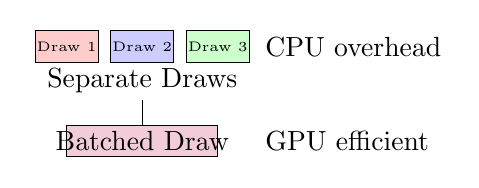
\begin{tikzpicture}[scale=0.8]
    % Draw call batching diagram
    \draw[fill=red!20] (0,0) rectangle (1,0.5);
    \node at (0.5,0.25) {\tiny Draw 1};
    \draw[fill=blue!20] (1.2,0) rectangle (2.2,0.5);
    \node at (1.7,0.25) {\tiny Draw 2};
    \draw[fill=green!20] (2.4,0) rectangle (3.4,0.5);
    \node at (2.9,0.25) {\tiny Draw 3};
    
    \node at (1.7, -0.3) {Separate Draws};
    
    \draw[->] (1.7, -0.6) -- (1.7, -1.2);
    
    \draw[fill=purple!20] (0.5,-1.5) rectangle (2.9,-1);
    \node at (1.7,-1.25) {Batched Draw};
    
    \node[right] at (3.5, 0.25) {CPU overhead};
    \node[right] at (3.5, -1.25) {GPU efficient};
\end{tikzpicture}
\end{center}

\end{frame}

\begin{frame}
\frametitle{Hardware Considerations}

\begin{mathbox}{Fixed-Function Hardware Units}
\begin{itemize}
    \item \textbf{Raster Units}: Triangle setup and pixel generation
    \item \textbf{ROP Units}: Render Output Pipeline (blending, depth test)
    \item \textbf{Texture Units}: Filtering and sampling hardware
    \item \textbf{Primitive Assembly}: Geometry processing
\end{itemize}
\end{mathbox}

\begin{center}
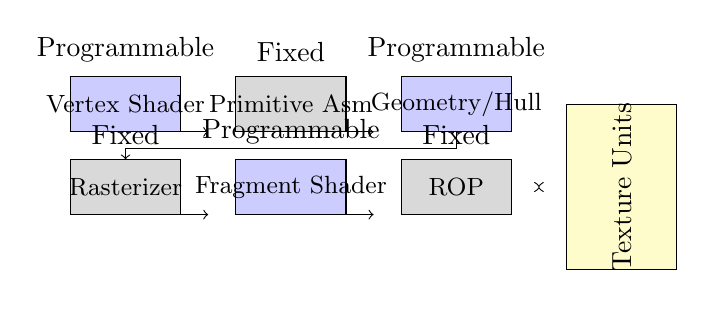
\begin{tikzpicture}[scale=0.7]
    % Modern GPU pipeline with hardware units
    \draw[fill=blue!20] (0,3) rectangle (2,4);
    \node at (1,3.5) {\small Vertex Shader};
    \node[above] at (1,4.1) {Programmable};
    
    \draw[fill=gray!30] (3,3) rectangle (5,4);
    \node at (4,3.5) {\small Primitive Asm};
    \node[above] at (4,4.1) {Fixed};
    
    \draw[fill=blue!20] (6,3) rectangle (8,4);
    \node at (7,3.5) {\small Geometry/Hull};
    \node[above] at (7,4.1) {Programmable};
    
    \draw[fill=gray!30] (0,1.5) rectangle (2,2.5);
    \node at (1,2) {\small Rasterizer};
    \node[above] at (1,2.6) {Fixed};
    
    \draw[fill=blue!20] (3,1.5) rectangle (5,2.5);
    \node at (4,2) {\small Fragment Shader};
    \node[above] at (4,2.6) {Programmable};
    
    \draw[fill=gray!30] (6,1.5) rectangle (8,2.5);
    \node at (7,2) {\small ROP};
    \node[above] at (7,2.6) {Fixed};
    
    % Arrows
    \draw[->] (1.5,3) -- (2.5,3);
    \draw[->] (4.5,3) -- (5.5,3);
    \draw[->] (7,3) -- (7,2.7) -- (1,2.7) -- (1,2.5);
    \draw[->] (1.5,1.5) -- (2.5,1.5);
    \draw[->] (4.5,1.5) -- (5.5,1.5);
    
    % Texture units
    \draw[fill=yellow!20] (9,0.5) rectangle (11,3.5);
    \node[rotate=90] at (10,2) {Texture Units};
    \draw[<->] (8.5,2) -- (8.5,2);
\end{tikzpicture}
\end{center}

\end{frame}

\begin{frame}
\frametitle{Performance Bottlenecks}

\begin{conceptbox}{Common Bottlenecks}
\begin{itemize}
    \item \textbf{Vertex-bound}: Too many vertices or complex vertex shaders
    \item \textbf{Fragment-bound}: High resolution or complex fragment shaders
    \item \textbf{Memory-bound}: Texture bandwidth or memory latency
    \item \textbf{CPU-bound}: Draw call overhead or game logic
\end{itemize}
\end{conceptbox}

\vspace{0.5cm}

\begin{center}
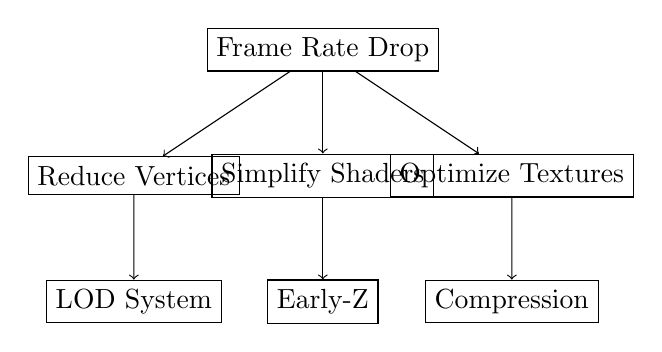
\begin{tikzpicture}[scale=0.8]
    % Performance analysis flowchart
    \node[draw, rectangle] (start) at (0,4) {Frame Rate Drop};
    
    \node[draw, rectangle] (vertex) at (-3,2) {Reduce Vertices};
    \node[draw, rectangle] (fragment) at (0,2) {Simplify Shaders};
    \node[draw, rectangle] (memory) at (3,2) {Optimize Textures};
    
    \node[draw, rectangle] (lod) at (-3,0) {LOD System};
    \node[draw, rectangle] (early) at (0,0) {Early-Z};
    \node[draw, rectangle] (compress) at (3,0) {Compression};
    
    \draw[->] (start) -- (vertex);
    \draw[->] (start) -- (fragment);
    \draw[->] (start) -- (memory);
    
    \draw[->] (vertex) -- (lod);
    \draw[->] (fragment) -- (early);
    \draw[->] (memory) -- (compress);
\end{tikzpicture}
\end{center}

\end{frame}
